
\section{NoSQL Databases}

\begin{breakbox}
\boxtitle{Scaling:}
\begin{itemize}
	\item Scale vertically (scale up):
		\begin{itemize}
			\item add resources to single node in a system, typically involving the addition of CPUs or memory to single computer.
		\end{itemize}
	\item Scale horizontally (scale out):
		\begin{itemize}
			\item add more nodes to a system, such as adding new computer to distributed software application.
		\end{itemize}
\end{itemize}
\end{breakbox}

\begin{breakbox}
\boxtitle{CAP Theorem:}
\begin{itemize}
	\item \textcolor{Emerald}{C}osistency: The data is in every replication on every server the same.
	\item \textcolor{Emerald}{A}vailability: The data must be always available (accessible).
	\item \textcolor{Emerald}{P}artition Tolerance: The db works fine despite network and machine failures.
\end{itemize}
One can only pick two of those properties at a time.
\end{breakbox}

\begin{breakbox}
\boxtitle{Consistency:}
\begin{itemize}
	\item Strong consistency:
		\begin{itemize}
			\item after an update is committed, each subsequent access will return the updated value.
		\end{itemize}
	\item Weak consistency:
		\begin{itemize}
			\item the systems does not guarantee that subsequent accesses will return the updated value.
			\item a number of conditions might need to be met before the updated value is returned.
			\item inconsistency window: period between update and the point in time when every access is guaranteed to return the updated value.
		\end{itemize}
	\item Eventual consistency:
		\begin{itemize}
			\item Specific form of weak consistency.
			\item If no new updates are made, eventually all accesses will return the last updated values.
			\item In the absence of failures, the maximum size of the inconsistency window can be determined based on communication delays, system load and number of replicas.
			\item Domain Name System (DNS) uses eventual consistency for updates.
			\item RDBMS use eventual consistency for asynchronous replication or backup.
		\end{itemize}
\end{itemize}
\end{breakbox}

\begin{breakbox}
\boxtitle{BASE:}
\begin{itemize}
	\item \textcolor{Emerald}{B}asically \textcolor{Emerald}{A}vailable: permanent availablity
	\item \textcolor{Emerald}{S}oft State: consistency is no solid state
	\item \textcolor{Emerald}{E}ventual Consistency: data is consistent sometime
\end{itemize}
\end{breakbox}

\begin{breakbox}
\boxtitle{NoSQL Characteristics:}
\begin{enumerate}
	\item Horizontal scalable (shared nothing)
	\item Can Replicate and distribute (partition) data
	\item Have simple API (no SQL binding)
	\item Have weaker concurrency / transaction model than ACID (eventually consistent)
	\item Are schema free, have weak schema restrictions (can add new attribues at runtime)
	\item Use distributed indexes and use RAM for data storage efficiently
\end{enumerate}
\end{breakbox}

\begin{breakbox}
\boxtitle{NoSQL Categories:}
\begin{enumerate}
	\item Key/Value databases
	\item Document stores
	\item Column oriented databases
	\item Graph databases
	\item Others
\end{enumerate}
\end{breakbox}

\begin{breakbox}
\boxtitle{Key/Value Databases:}
\begin{itemize}
	\item Key/Value Pairs:
		\begin{itemize}
			\item Key-value pairs (KVP), dictionary or associative array, map, hash.
			\item An Abstract Data Structure (ADT). Most modern scripting languages support dictionaries/associative arrays as a primary container type.
			\item Hstore in PostgreSQL. Oracle has associative arrays in PL/SQL (through functions, not []).
		\end{itemize}
	\item In memory or on disk
	\item Examples: Redis, SimpleDB (on disk), Membase (in memory), Tokyo Cabinet, Berkeley DB, Azure Table Storage
\end{itemize}
\end{breakbox}

\begin{breakbox}
\boxtitle{Document Stores:}
\begin{itemize}
	\item Similar to Key/Value databases but value is a document
	\item Flexible Schema
	\item Document stored in JSON or BSON formats
	\item Examples: MongoDB, CouchDB
\end{itemize}
\end{breakbox}

\begin{breakbox}
\boxtitle{PostgreSQL mit JSON(B):}
\begin{itemize}
	\item relational database and noSQL-document-store combined.
	\item JSON since PG 9.2:
		\begin{itemize}
			\item Save data as text, formatting and sequence of the elements are preserved.
			\item Checks if JSON-syntax is valid.
		\end{itemize}
	\item JSONB since PG 9.4:
		\begin{itemize}
			\item Save data as binary.
			\item keys have to be unique for same JSON-document (the last key will be used).
			\item Slower inserts, faster queries.
		\end{itemize}
	\item Expression index for special queries:
		\begin{itemize}
			\item \lstinline[language=SQL]{CREATE INDEX on movies_jsonb((movie#>>'{actors,0,lastname)'));}
			\item very fast queries on above attribute in WHERE-part.
		\end{itemize}
	\item Standard GIN-index (jsonb\_ops):
		\begin{itemize}
			\item \lstinline[language=SQL]{CREATE INDEX idx_ops on movies_jsonb USING gin (movie);}
			\item supports operators: @>, ?, ?\& and ?|
		\end{itemize}
	\item Non-standard GIN-index (json\_path\_ops):
		\begin{itemize}
			\item \lstinline[language=SQL]{CREATE INDEX idx_path_ops on movies_jsonb USING gin (movie jsonb_path_ops);}
			\item supports operator: @>
		\end{itemize}
\end{itemize}
\end{breakbox}

\begin{breakbox}
\boxtitle{MongoDB:}
\begin{itemize}
	\item Stores documents in BSON.
	\item Supports ad hoc queries against objects and arrays.
	\item Scales horizontally via sharding.
	\item Giery interface:
\end{itemize}
\begin{center}
	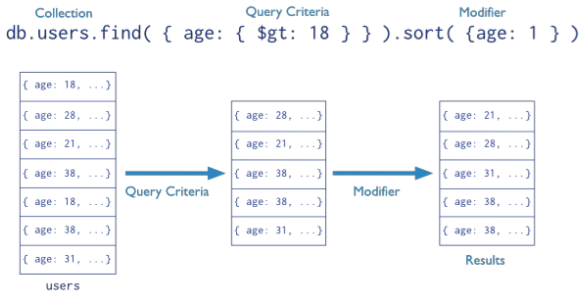
\includegraphics[width=.12\textwidth]{slides_images/mongo_db_query}
\end{center}
\begin{itemize}
	\item Indexes:
		\begin{itemize}
			\item Single field, Compund index
			\item Multikey index (<field>: <1 or -1>)
			\item Geospatial index
			\item Text indexes, Hashed indexes
		\end{itemize}
\end{itemize}
\end{breakbox}

\begin{breakbox}
\boxtitle{Column Oriented Databases:}
\begin{itemize}
	\item Wide Column Stores
	\item Each key is associated with multiple attributes
	\item Examples: HBase, Cassandra
\end{itemize}
\end{breakbox}

\begin{breakbox}
\boxtitle{HBase:}
\begin{itemize}
	\item Layered over Hadoop Distributed File System $\Rightarrow$ highly distributed.
	\item RESTful API
	\item Input/Output for MapReduce Jobs
	\item Automatic partitioning, re-balancing
\end{itemize}
\end{breakbox}

\begin{breakbox}
\boxtitle{Cassandra:}
\begin{itemize}
	\item Eventually consistent
	\item Designed for distributed databases
	\item Optimized for ring shaped clusters
	\item Columns hold name, values and time stamp
	\item Columns are sorted by key-name
\end{itemize}
\end{breakbox}

\begin{breakbox}
\boxtitle{MemSQL:}
\begin{itemize}
	\item In-memory database supporting disk-based column stores
	\item reference tables / shard tables
	\item Indexes:
		\begin{itemize}
			\item Skip lists (B-Tree)
			\item Column store
			\item Hash table
			\item Index commands: CREATE INDEX, DROP INDEX, SHOW INDEX, SHOW INDEXES, SHOW KEYS, EXPLAIN
		\end{itemize}
\end{itemize}
\end{breakbox}

\begin{breakbox}
\boxtitle{Graph Databases:}
\begin{itemize}
	\item Examples: Neo4j, FlockDB, InfiniteGraph
\end{itemize}
\end{breakbox}

\begin{breakbox}
\boxtitle{Neo4j:}
\begin{itemize}
	\item Data model: Property graph
	\item Primary operation: Traversal
	\item Disk-based
	\item Scales to billions of nodes per JVM
	\item Index: CREATE INDEX IN :Person(name)
\end{itemize}
\end{breakbox}

\begin{breakbox}
\boxtitle{Others:}
\begin{itemize}
	\item Object stores (db4o)
	\item In-memory stores
	\item Array stores
	\item Tree stores / XML databases (Tamino, eXist)
\end{itemize}
\end{breakbox}























